\documentclass[a4paper,12pt]{article}

% Packages
\usepackage{graphicx}   % For diagrams
\usepackage{geometry}   % Page layout
\usepackage{hyperref}   % Hyperlinks
\usepackage{titlesec}   % Formatting section titles
\usepackage{enumitem}   % Bullet points
\usepackage{caption}    % Figure captions
\usepackage{tikz}       % UML diagrams
\usetikzlibrary{positioning}

% Page setup
\geometry{left=2.5cm, right=2.5cm, top=2.5cm, bottom=2.5cm}

% Title Formatting
\titleformat{\section}{\Large\bfseries}{\thesection}{1em}{}

\begin{document}

% Title
\begin{center}
    {\LARGE \textbf{HCLI - Habit Tracker CLI}}\\[0.5cm]
    {\Large \textbf{Conception Phase}}\\[0.3cm]
    {\small Author: Alejandro Moral Aranda \hspace{1cm} Date: \today}
    \hrule
\end{center}

% Section: Introduction
\section{Introduction}
HCLI (Habit Tracker CLI) is a command-line-based habit tracking application that provides users with a lightweight, efficient, and distraction-free way to track their habits. Unlike traditional mobile or web-based applications, HCLI focuses on speed and usability through a command-line interface (CLI), allowing users to add, check, and analyze their habits through simple commands.

The goal of HCLI is to provide a seamless experience for users who prefer a terminal-driven workflow, ensuring that they can manage their habits without the need for graphical interfaces. This document outlines the technical foundation, system architecture, and workflow behind HCLI.

% Section: Core Functionalities
\section{Core Functionalities}
The HCLI application is designed with the following core functionalities:
\begin{itemize}
    \item Adding habits: Users can define habits with a name and periodicity (daily/weekly).
    \item Tracking progress: Users can mark habits as completed.
    \item Viewing streaks: The system calculates the longest streaks for each habit.
    \item Analytics and summaries: Users can analyze which habits they struggle with and view overall progress.
    \item Reminders: Displays pending habits that need to be completed.
    \item Dashboard: Provides visual analytics (ASCII or graphical).
    \item Configuration: Users can adjust file storage paths and customize settings.
\end{itemize}

% Section: User Interaction and Workflow
\section{User Interaction and Workflow}
The general user flow of HCLI is designed to be intuitive and efficient. The interaction follows a simple command-driven workflow:

\begin{enumerate}
    \item User initializes the application by setting up their username:
    \begin{verbatim}
    python main.py setup-user
    \end{verbatim}
    
    \item User adds a new habit specifying the habit name and periodicity:
    \begin{verbatim}
    python main.py add "Workout" daily
    \end{verbatim}
    
    \item User checks off a habit when completed:
    \begin{verbatim}
    python main.py check "Workout"
    \end{verbatim}

    \item User views analytics and streaks:
    \begin{verbatim}
    python main.py summary
    python main.py streaks
    \end{verbatim}

    \item User manages configuration:
    \begin{verbatim}
    python main.py config --show
    \end{verbatim}

    \item User accesses dashboard visualization:
    \begin{verbatim}
    python main.py dashboard
    \end{verbatim}
\end{enumerate}

% Section: Data Management
\section{Data Management}
All habit data is stored in JSON files to ensure simplicity and portability. The data files include:

\begin{itemize}
    \item \textbf{habits.json} - Stores user habits, their periodicity, and timestamps.
    \item \textbf{user.json} - Stores user preferences, including the username.
    \item \textbf{config.json} - Stores the application configuration settings.
\end{itemize}

% Section: System Architecture
\section{System Architecture}
The HCLI application consists of several key components:

\begin{itemize}
    \item CLI Interface: Handles user input and executes commands.
    \item Data Management: Reads and writes habit data to JSON.
    \item Analytics Engine: Calculates streaks, summaries, and habit trends.
    \item Reminder System: Checks for pending habits.
    \item Dashboard: Provides ASCII or graphical visualizations.
\end{itemize}

\begin{center}
\begin{figure}[h]
    \centering
    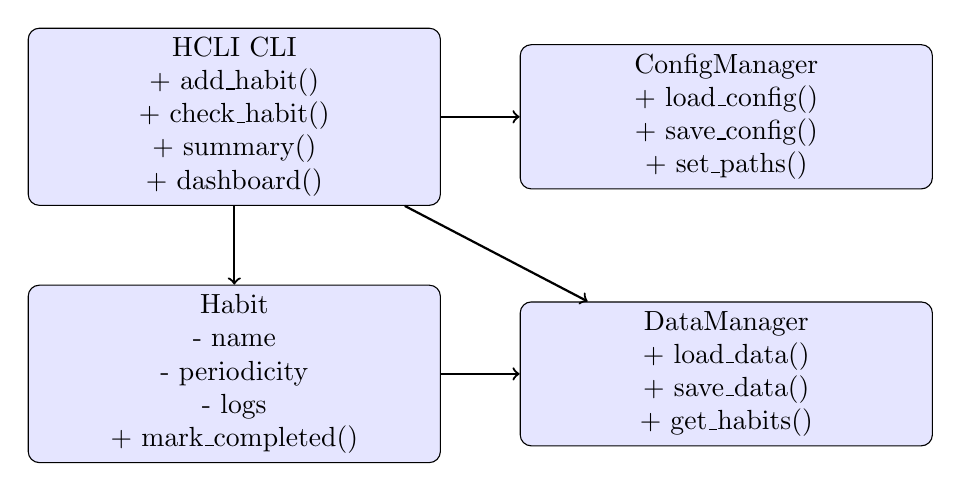
\begin{tikzpicture}[
        class/.style={rectangle, draw, fill=blue!10, rounded corners, text width=5cm, minimum height=1.5cm, align=center},
        interface/.style={rectangle, draw, fill=red!10, dashed, text width=5cm, minimum height=1.5cm, align=center},
        arrow/.style={->, thick}
    ]

    % Classes
    \node[class] (cli) {HCLI CLI \\ + add\_habit() \\ + check\_habit() \\ + summary() \\ + dashboard()};
    \node[class, below=of cli] (habit) {Habit \\ - name \\ - periodicity \\ - logs \\ + mark\_completed()};
    \node[class, right=of habit] (data) {DataManager \\ + load\_data() \\ + save\_data() \\ + get\_habits()};
    \node[class, right=of cli] (config) {ConfigManager \\ + load\_config() \\ + save\_config() \\ + set\_paths()};

    % Relationships
    \draw[arrow] (cli) -- (habit);
    \draw[arrow] (cli) -- (data);
    \draw[arrow] (cli) -- (config);
    \draw[arrow] (habit) -- (data);

    \end{tikzpicture}
    \caption{UML Class Diagram for HCLI}
\end{figure}
\end{center}

% Section: Tools and Technologies
\section{Tools and Technologies}
HCLI is implemented using the following technologies:

\begin{itemize}
    \item Python - The core programming language.
    \item Typer - Used for handling CLI commands.
    \item Rich - Provides colorful terminal output and tables.
    \item JSON - Stores persistent data for habits and user preferences.
    \item Pytest - Used for unit testing the application.
\end{itemize}

% Section: Implementation Plan
\section{Implementation Plan}
The development of HCLI follows a structured roadmap:
\begin{itemize}
    \item Phase 1: Core functionality (add, check, list habits).
    \item Phase 2: Advanced features (analytics, reminders, streaks).
    \item Phase 3: Optimization, visualization, and testing.
\end{itemize}

% Section: Conclusion
\section{Conclusion}
HCLI is a lightweight, efficient, and terminal-based habit tracking solution designed for users who prefer CLI-driven workflows. By leveraging simple commands, structured data management, and insightful analytics, HCLI provides a seamless experience for habit formation and tracking. This document lays the foundation for development, ensuring a well-structured implementation and feature roadmap.

\end{document}
